

%----------------------------------------------------------------------------------------
%	PACKAGES AND OTHER DOCUMENT CONFIGURATIONS
%----------------------------------------------------------------------------------------

\documentclass[12pt]{article} % Default font size is 12pt, it can be changed here

\usepackage[utf8]{inputenc}
\usepackage{indentfirst}
\usepackage{geometry} % Required to change the page size to A4
\geometry{a4paper} % Set the page size to be A4 as opposed to the default US Letter

\usepackage{graphicx} % Required for including pictures

\usepackage{float} % Allows putting an [H] in \begin{figure} to specify the exact location of the figure
\usepackage{wrapfig} % Allows in-line images such as the example fish picture

\usepackage{lipsum} % Used for inserting dummy 'Lorem ipsum' text into the template

\linespread{1.2} % Line spacing

%\setlength\parindent{0pt} % Uncomment to remove all indentation from paragraphs

\graphicspath{{Pictures/}} % Specifies the directory where pictures are stored

\begin{document}

%----------------------------------------------------------------------------------------
%	TITLE PAGE
%----------------------------------------------------------------------------------------

\begin{titlepage}

\setcounter{secnumdepth}{5}

\newcommand{\HRule}{\rule{\linewidth}{0.5mm}} % Defines a new command for the horizontal lines, change thickness here

\center % Center everything on the page

\textsc{\LARGE Bilkent University}\\[1.5cm] % Name of your university/college
\textsc{\Large Group: 1G}\\[0.5cm] % Major heading such as course name
\textsc{\large Design Report Draft}\\[0.5cm] % Minor heading such as course title

\HRule \\[0.4cm]
{ \huge \bfseries Emoji Strike }\\ % Title of your document
\HRule \\[1.5cm]

\begin{minipage}{0.4\textwidth}
\begin{flushleft} \large
\emph{Author:}\\
Ali \textsc{Salemwala} 
\\ Bora \textsc{Bardük}
\\ Eren \textsc{Çalık}
\\ Kıvanç \textsc{Gümüş}
\end{flushleft}
\end{minipage}
~
\begin{minipage}{0.4\textwidth}
\begin{flushright} \large
\emph{Supervisor:} \\
Bora \textsc{Güngören} % Supervisor's Name
\end{flushright}
\end{minipage}\\[4cm]

{\large \today}\\[3cm] % Date, change the \today to a set date if you want to be precise

%\includegraphics{Logo}\\[1cm] % Include a department/university logo - this will require the graphicx package

\vfill % Fill the rest of the page with whitespace

\end{titlepage}

%----------------------------------------------------------------------------------------
%	TABLE OF CONTENTS
%----------------------------------------------------------------------------------------

\tableofcontents % Include a table of contents

\newpage % Begins the essay on a new page instead of on the same page as the table of contents 

%----------------------------------------------------------------------------------------
%	INTRODUCTION
%----------------------------------------------------------------------------------------

\section{Introduction} % Major section

%------------------------------------------------

\subsection{Purpose of the System} % Sub-section


Emoji Strike is a 2-D arcade game. The game is designed so that a group of friends can have good a time playing the game on the same device competitively. The game firstly introduces the user with a brief tutorial to teach the user how the game is played. As the user(s) decide that they have learned this gameplay and controls, they move on to the game building stage which includes user’s picking their desired character and map of choice. When this game building stage is done users can enjoy the game they built for themselves until one of the them becomes the victor. Therefore, our main purpose is to design a dynamic and a competitive game.


%------------------------------------------------

\subsection{Design Goals } % Sub-section


%------------------------------------------------


\input{inputs/input1.txt}

%------------------------------------------------


%----------------------------------------------------------------------------------------


%----------------------------------------------------------------------------------------


%----------------------------------------------------------------------------------------

\subsection{Definitions, Acronyms, Abbreviations} % Sub-section

%----------------------------------------------------------------------------------------

\subsection{References} % Sub-section

%----------------------------------------------------------------------------------------

%----------------------------------------------------------------------------------------

\subsection{Overview} % Sub-section

%----------------------------------------------------------------------------------------
% 	SOFTWARE ARCHITECTURE
%----------------------------------------------------------------------------------------

\section{Software Architecture} % Major section

%------------------------------------------------

\subsection{Overview} % Sub-section

This section will decompose our program into smaller, more manageable parts, so that it may be built more efficiently and cleanly. Additionally, partitioning the sections will mean that the different program parts will not interfere with each other, and one misbehaving section may not disturb other sections. We will try to use a Model-View-Controller style architecture on our program.

%------------------------------------------------

\subsection{Subsystem Decomposition} % Sub-section

To ensure that our system contains maintanable, discrete, independant sections, we will break it up into 3 section: mainly the User Interface Section, which will serves as the view, the Game Management Section, which serves as the controller, and the Game system itself, which is the model. This way, we can not only independantly develop the sections, but also prevent bugs from one section from leaking into others. Additionally, our code will remain maintainable in the future, since related functionalities will be grouped together and the future maintainers will have a well-documented and partitioned system to maintain.
\indent Below are diagrams indicating how the system and actions inside it are divided up. They can serve not only as guidelines while the system is being developed, but also as references for the future when the system is already running.

%------------------------------------------------

\subsection{Architectural Styles} % Sub-section

%------------------------------------------------

\subsubsection{Layers} % Subsub-section

This system has been divided into three layers, which are closely mirrored by the MVC-style architectre the entire program follows. The top-most layer, the User-Interface Layer, is the one that is in direct contact with the user. It is the only layer which the user is allowed to directly influence. Beneath this comes the Game Management layer, which is synonomous to the Game Management subsystem. This can only be influenced by the User Interface layer, and directly influences the Game layer. It serves as a pipeline between what the user sees and the actual system, and transfers any changes from one end to the other. Finally, comes the Game layer, which can be considered to be the engine of the entire system. It is the actual state of the system, and is altered directly by the Game Management layer. Changes are passed back through the same layer. This layered system has been created to prevent any undue influencing of the system by the user, so that only appropriate layers can be changed, and these changes are done in a controlled, pre-decided manner.

%------------------------------------------------

\subsubsection{Model View Controller} % Subsub-section

The Model-View-Controller style serves as a complement to the layer sytle described above. It divides the system into the Model, which cannot be altered directly by anybody except the Controller, which is merged with the View to display the whole program to the user. Since our program is a gme, it is especially useful for our system to be divided as an MVC-style architecture, since the game state must be influenced only by the user, but must also not be freely changed, and should instead have a controlled pathway for changes to take the proper effect.

%------------------------------------------------

\subsection{Hardware/Software Mapping} % Sub-section

EmojiStrike will be implemented in Java, and will use JDK 1.8. The hardware used are a keyboard, speakers, and the monitor display. The software needed is only an operating systme which can run the .jar file which will contain our game. Storage will be done in .txt format, so the operating system should be able to store the saved files.

%------------------------------------------------

\subsection{Persistent Data Management} % Sub-section

The game does not have any complex or detailed information that needs to be stored. The default maps will be stored, and the edited versions with other game details will be stored as individual files. The game will be able to function if the saved files are corrupted, although the saved game will obviously be lost. Sound files and images for the emojis, weapons, and animations will also be stored, and if these are corrupted, the game will experience significant problems.

%------------------------------------------------

\subsection{Access Control and  Security} % Sub-section

There are no network or security requirements for this game.

%------------------------------------------------

\subsection{Boundary Conditions} % Sub-section
Below is a list of boundary conditions in our application.\\
\textbf{Initialization:} There is no need for any installation. Simply running the main .jar file is enough to run the game, as long as the system has Java installed.\\
\textbf{Termination:} The system can exit with a simple keypress, both with or without saving the game. Saving the game will also require the user to enter a name for the current game.\\
\textbf{Error:} The game may not load saved games if the files are corrupted.\\
The game may not load certain images or sounds if the files are corrupted.\\
		An error while playing the game might cause the entire system to shut down, but we will try to include ways to handle all errors and maintain user experience.\\

%----------------------------------------------------------------------------------------
%	Subsystem Design
%----------------------------------------------------------------------------------------

\section{Subsystem Design} % Major section

In this section, we will bridge the gap between a problem and an existing system in a manageable way by using divide and conquer approach.

\subsection{Architectural Style}

\subsubsection{Model View Controller Design}
\input{inputs/mvc.txt}

\subsection{User Interface Subsystem}

Figure \ref{fig:views} illustrates the User Interface Management Subsystem Diagram.
\begin{figure}[h!]
   \centering
   \vspace{10pt}%
   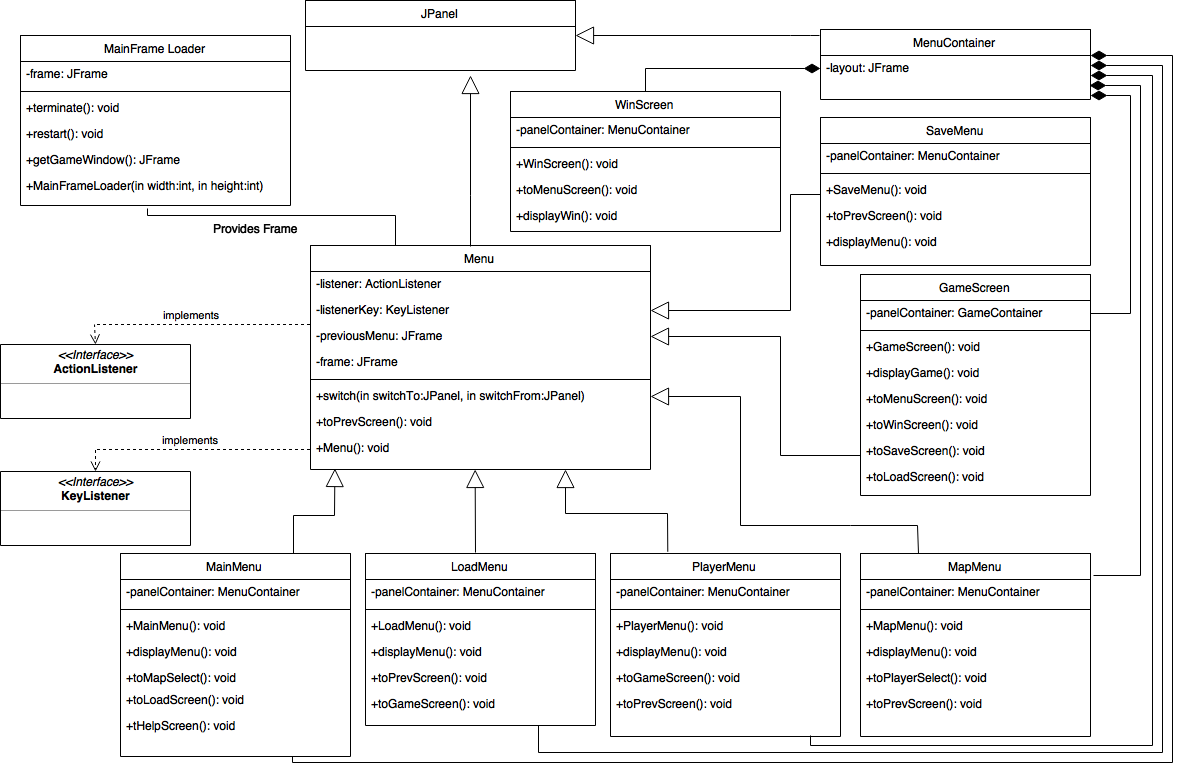
\includegraphics[width=17cm]{views.png}
   \caption{User Interface Management Subsystem}
   \label{fig:views}
\end{figure}

User Interface Management Subsystem consists of 11 classes which contains the views and information necessary to establish communication between users and Emoji Strike.  There are two interfaces implemented and used during the design of out interface.  These classes and their properties will be discussed in-depth in the following sections.

%menu
\subsubsection{Menu}

Figure \ref{fig:menu} illustrates the Menu Class.
\begin{figure}[h!]
   \centering
   \vspace{10pt}%
   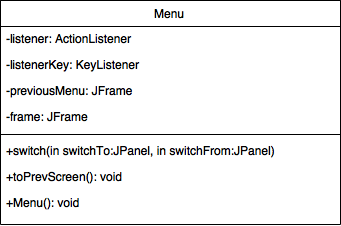
\includegraphics[width=10cm]{menu.png}
   \caption{Menu Class}
   \label{fig:menu}
\end{figure}

\paragraph{Attributes \\}

List of attributes used in Menu class.\\
\textbf{private JFrame frame:} All visuals of the window will be displayed here.\\
\textbf{private KeyListener listenerKey:} Our users will provide input to Emoji Strike using keyboard buttons. \\
\textbf{private ActionListener listener:} When a certain menu button is activated, this listener will retrieve the activated object to perform related operations.\\
\textbf{private JFrame previousMenu:} This attribute will contain the last accessed JFrame before the current one.  This is used to provide "go back" function to any screen in the game.

\paragraph{Constructors \\}
List of constructors used in Menu class.\\
\textbf{public Menu:} Initializes frame, listener, listenerKey, previousMenu which are the attributes of Menu class.

\paragraph{Operations \\}
List of operations used in Menu class.\\
\textbf{public void switch:} Used to switch between different panel instances.\\
\textbf{public void toPrevScreen:} Used to switch to the previous screen by accessing the private attribute \textit{previousMenu}.
%/menu

%mainf loader
\subsubsection{MainFrame Loader}

Figure \ref{fig:loader} illustrates the MainFrameLoader Class.
\begin{figure}[h!]
   \centering
   \vspace{10pt}%
   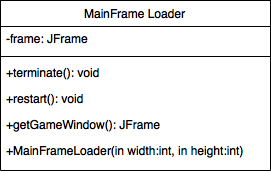
\includegraphics[width=10cm]{loader.png}
   \caption{MainFrame Loader Class}
   \label{fig:mainframeloader}
\end{figure}

\paragraph{Attributes \\}

List of attributes used in MainFrameLoader class.\\
\textbf{private JFrame frame:} Opens up the main screen which will then be used by the Menu class and its panels.  All visuals of the window will be displayed here.\\

\paragraph{Constructors \\}
List of constructors used in MainFrameLoader class.\\
\textbf{public MainFrameLoader:} Initializes frame which is the attribute of MainMenuLoader class.  It consists of parameters width and height, which will be the screen resolution determined for a display.

\paragraph{Operations \\}
List of operations used in MainFrameLoader class.\\
\textbf{public JFrame getGameWindow:} Returns the JFrame object which will be displayed on the screen.
\textbf{public void terminate:} Used to terminate the main screen instance when operations like \textit{quit} are performed.\\
\textbf{public void restart:} Used to restart the main frame of the game when user prompts.
%/mainf loader

%mainmenu
\subsubsection{MainMenu}

Figure \ref{fig:mainmenu} illustrates the MainMenu Class.
\begin{figure}[h!]
   \centering
   \vspace{10pt}%
   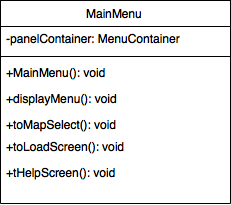
\includegraphics[width=10cm]{mainmenu.png}
   \caption{MainMenu Class}
   \label{fig:mainmenu}
\end{figure}

\paragraph{Attributes \\}

List of attributes used in MainMenu class.\\
\textbf{private MenuContainer panelContainer:} The container which holds the graphical elements of the MainMenu class.

\paragraph{Constructors \\}
List of constructors used in MainMenu class.\\
\textbf{public MainMenu:} Initializes panel which is the attribute of MainMenu class.

\paragraph{Operations \\}
List of operations used in MainMenu class.\\
\textbf{public JFrame getGameWindow:} Returns the JFrame object which will be displayed on the screen.\\
\textbf{public void displayMenu:} Used to load the graphical elements after the instance of the class is created.\\
\textbf{public void toMapSelect:} Switches the panel view to \textit{MapSelectMenu} which is where user selects the map to play the game on.\\
\textbf{public void toLoadScreen:} Switches the panel view to \textit{LoadMenu} which is where user selects from the previous game files saved.\\
\textbf{public void tHelpScreen:} Toggles the graphical elements which will load the \textit{How to play} instructions.
%/mainmenu load

%LoadMenu
\subsubsection{LoadMenu} %image is not in the right place, because latex doesn't want to waste page

Figure \ref{fig:loadmenu} illustrates the LoadMenu Class.
\begin{figure}[h!]
   \centering
   \vspace{10pt}%
   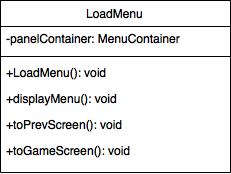
\includegraphics[width=10cm]{loadmenu.png}
   \caption{LoadMenu Class}
   \label{fig:loadmenu}
\end{figure}

\paragraph{Attributes \\}

List of attributes used in LoadMenu class.\\
\textbf{private MenuContainer panelContainer:} The container which holds the graphical elements of the LoadMenu class. 


\paragraph{Constructors \\}
List of constructors used in LoadMenu class.\\
\textbf{public LoadMenu:} Initializes panel which is the attribute of LoadMenu class.


\paragraph{Operations \\}
List of operations used in LoadMenu class.\\
\textbf{public void displayMenu:} Used to load the graphical elements after the instance of the class is created.\\
\textbf{public void toPrevScreen:} Used to switch to the previous screen by accessing the private attribute \textit{previousMenu}.\\
\textbf{public void toGameScreen:} After the the load file is prompted by the user, the information is initialized to appear in \textit{GameScreen}.

%/LoadMenu

%PlayerMenu
\subsubsection{PlayerMenu} %image is not in the right place, because latex doesn't want to waste page

Figure \ref{fig:playermenu} illustrates the PlayerMenu Class.
\begin{figure}[h!]
   \centering
   \vspace{10pt}%
   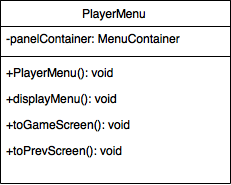
\includegraphics[width=10cm]{playermenu.png}
   \caption{PlayerMenu Class}
   \label{fig:playermenu}
\end{figure}

\paragraph{Attributes \\}

List of attributes used in PlayerMenu class.\\
\textbf{private MenuContainer panelContainer:} The container which holds the graphical elements of the PlayerMenu class. 

\paragraph{Constructors \\}
List of constructors used in PlayerMenu class.\\
\textbf{public PlayerMenu:} Initializes panel which is the attribute of PlayerMenu class.


\paragraph{Operations \\}
List of operations used in PlayerMenu class.\\
\textbf{public void displayMenu:} Used to load the graphical elements after the instance of the class is created.\\
\textbf{public void toPrevScreen:} Used to switch to the previous screen by accessing the private attribute \textit{previousMenu}.\\
\textbf{public void toGameScreen:} After the players are initialized, the information is directed to appear in \textit{GameScreen}.

%/PlayerMenu


%MapMenu
\subsubsection{MapMenu} %image is not in the right place, because latex doesn't want to waste page

Figure \ref{fig:mapmenu} illustrates the MapMenu Class.
\begin{figure}[h!]
   \centering
   \vspace{10pt}%
   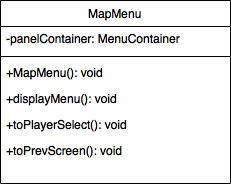
\includegraphics[width=10cm]{mapmenu.png}
   \caption{MapMenu Class}
   \label{fig:mapmenu}
\end{figure}

\paragraph{Attributes \\}

List of attributes used in MapMenu class.\\
\textbf{private MenuContainer panelContainer:} The container which holds the graphical elements of the MapMenu class. 

\paragraph{Constructors \\}
List of constructors used in MapMenu class.\\
\textbf{public MapMenu:} Initializes panel which is the attribute of MapMenu class.


\paragraph{Operations \\}
List of operations used in MapMenu class.\\
\textbf{public void displayMenu:} Used to load the graphical elements after the instance of the class is created.\\
\textbf{public void toPrevScreen:} Used to switch to the previous screen by accessing the private attribute \textit{previousMenu}.\\
\textbf{public void toPlayerSelect:} After the map is selected, user is directed to enter player information for them to appear in the \textit{GameScreen}.

%/MapMenu


%SaveMenu
\subsubsection{SaveMenu} %image is not in the right place, because latex doesn't want to waste page

Figure \ref{fig:savemenu} illustrates the SaveMenu Class.
\begin{figure}[h!]
   \centering
   \vspace{10pt}%
   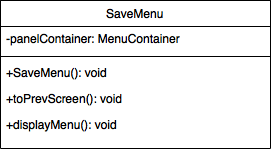
\includegraphics[width=10cm]{savemenu.png}
   \caption{SaveMenu Class}
   \label{fig:savemenu}
\end{figure}

\paragraph{Attributes \\}

List of attributes used in SaveMenu class.\\
\textbf{private MenuContainer panelContainer:} The container which holds the graphical elements of the SaveMenu class. 

\paragraph{Constructors \\}
List of constructors used in SaveMenu class.\\
\textbf{public SaveMenu:} Initializes panel which is the attribute of SaveMenu class.


\paragraph{Operations \\}
List of operations used in SaveMenu class.\\
\textbf{public void displayMenu:} Used to load the graphical elements after the instance of the class is created.\\
\textbf{public void toPrevScreen:} Used to switch to the previous screen by accessing the private attribute \textit{previousMenu}.

%/SaveMenu


%GameScreen
\subsubsection{GameScreen} %image is not in the right place, because latex doesn't want to waste page

Figure \ref{fig:gamescreen} illustrates the GameScreen Class.
\begin{figure}[h!]
   \centering
   \vspace{10pt}%
   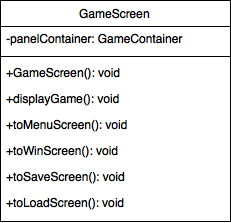
\includegraphics[width=10cm]{gamescreen.png}
   \caption{GameScreen Class}
   \label{fig:gamescreen}
\end{figure}

\paragraph{Attributes \\}

List of attributes used in GameScreen class.\\
\textbf{private MenuContainer panelContainer:} The container which holds the graphical elements of the GameScreen class. 

\paragraph{Constructors \\}
List of constructors used in GameScreen class.\\
\textbf{public GameScreen:} Initializes panel which is the attribute of GameScreen class.

\paragraph{Operations \\}
List of operations used in GameScreen class.\\
\textbf{public void displayGame:} Used to load the graphical elements after the instance of the class is created.\\
\textbf{public void toMenuScreen:} Used to immediately return to the view panel store in \textit{MainMenu}. \\
\textbf{public void toWinScreen:} After the winner is determined, this operation is used to switch to view \textit{WinScreen}. \\
\textbf{public void toLoadScreen:} Switches the panel view to \textit{LoadMenu} which is where user selects from the previous game files saved.\\
\textbf{public void toSaveScreen:} Switches the panel view to \textit{LoadMenu} which is where user selects from the previous game files saved.\\

%/GameScreen


%WinScreen
\subsubsection{WinScreen} %image is not in the right place, because latex doesn't want to waste page

Figure \ref{fig:winscreen} illustrates the WinScreen Class.
\begin{figure}[h!]
   \centering
   \vspace{10pt}%
   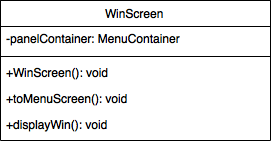
\includegraphics[width=10cm]{winscreen.png}
   \caption{WinScreen Class}
   \label{fig:winscreen}
\end{figure}

\paragraph{Attributes \\}

List of attributes used in WinScreen class.\\
\textbf{private MenuContainer panelContainer:} The container which holds the graphical elements of the GameScreen class. 

\paragraph{Constructors \\}
List of constructors used in WinScreen class.\\
\textbf{public WinScreen:} Initializes panel which is the attribute of WinScreen class.

\paragraph{Operations \\}
List of operations used in GameScreen class.\\
\textbf{public void displayWin:} Used to load the graphical elements after the instance of the class is created.\\
\textbf{public void toMenuScreen:} Used to immediately return to the view panel store in \textit{MainMenu}. \\

%/WinScreen


%MenuContainer
\subsubsection{MenuContainer} %image is not in the right place, because latex doesn't want to waste page

Figure \ref{fig:menucontainer} illustrates the MenuContainer Class.
\begin{figure}[h!]
   \centering
   \vspace{10pt}%
   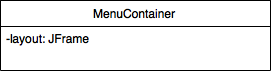
\includegraphics[width=10cm]{menucontainer.png}
   \caption{MenuContainer Class}
   \label{fig:menucontainer}
\end{figure}

\paragraph{Attributes \\}

List of attributes used in MenuContainer class.\\
\textbf{private JFrame layout:} All visuals of the window will be displayed here\\


%/MenuContainer


%entitites
\subsection{Entities Subsystem}

Figure \ref{fig:entity} illustrates the Entites Subsystem Diagram.

\begin{figure}[h!]
   \centering
   \vspace{10pt}%
   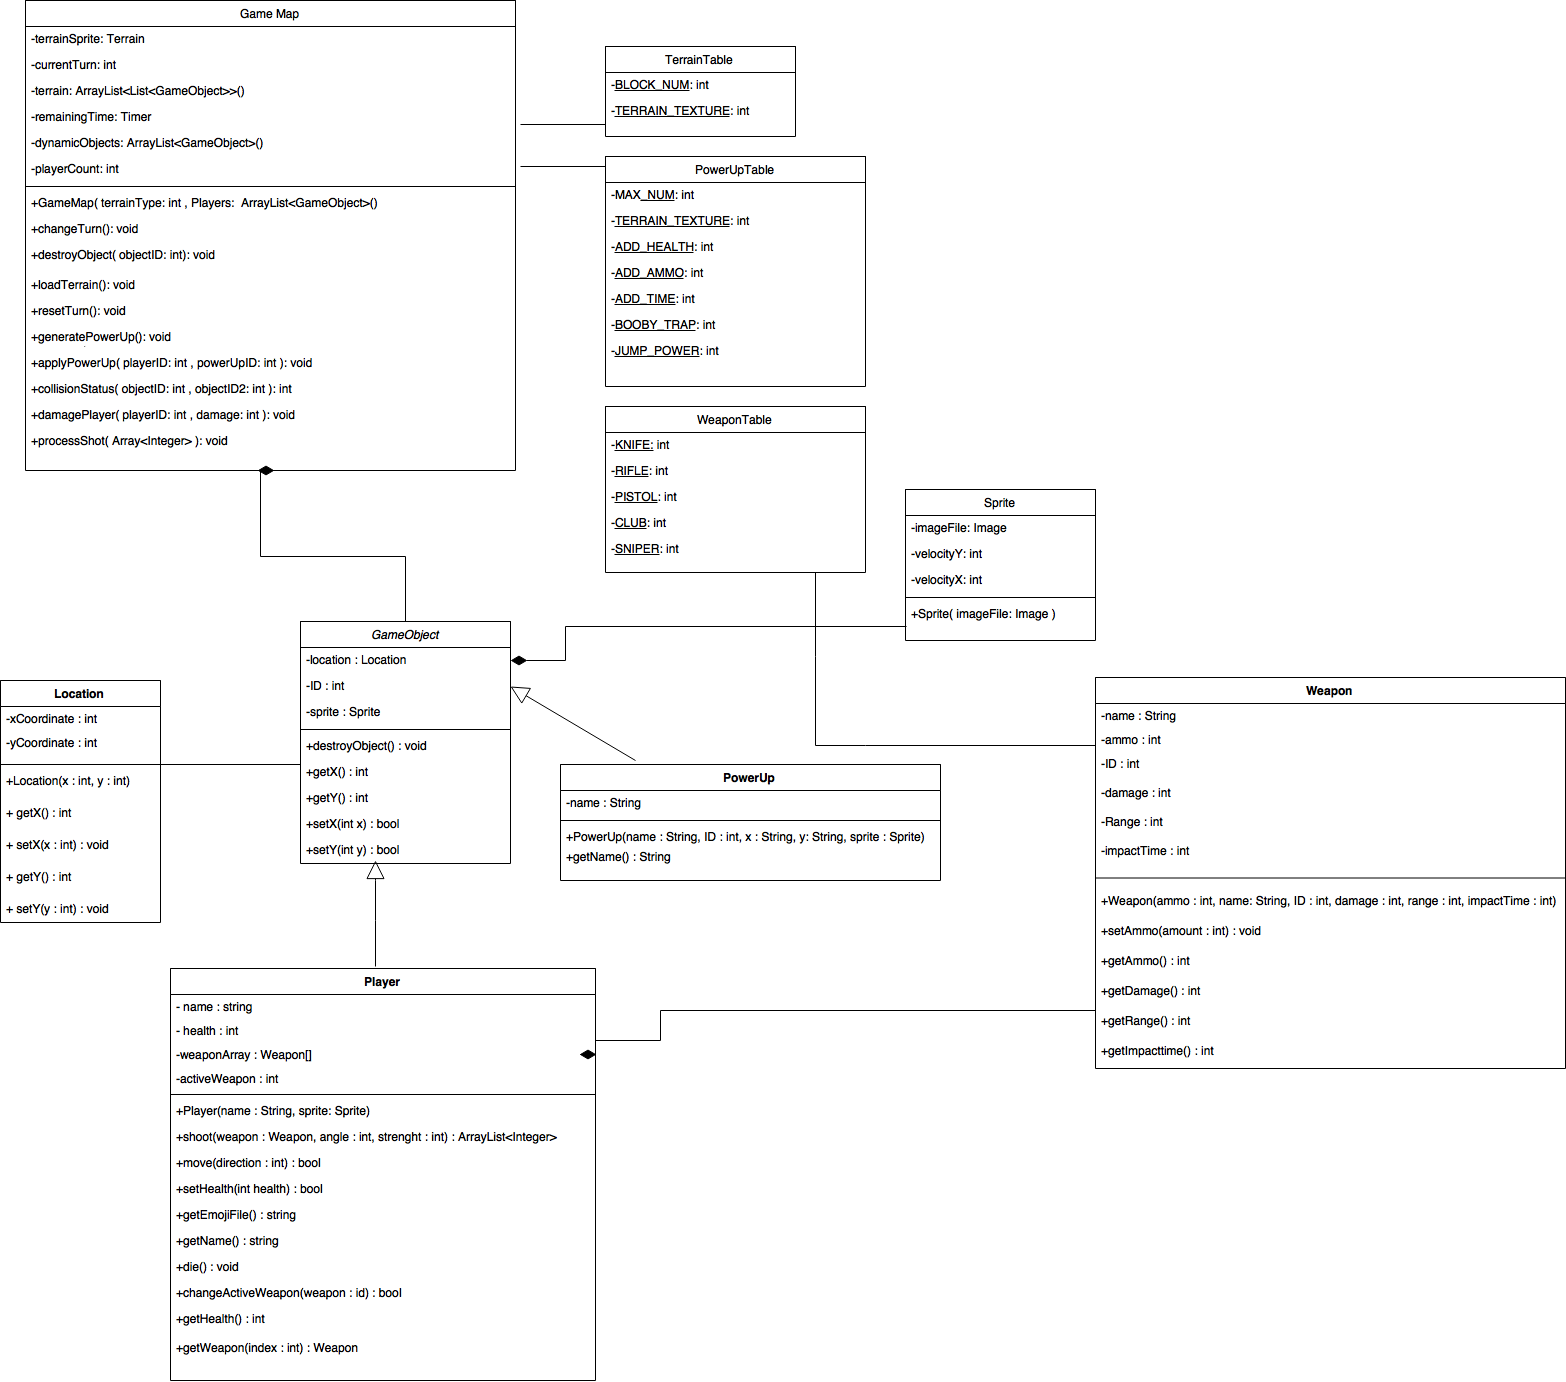
\includegraphics[width=17cm]{entity.png}
   \caption{Entities Subsystem}
   \label{fig:entity}
\end{figure}

%GameMap
\subsubsection{GameMap} %image is not in the right place, because latex doesn't want to waste page

Figure \ref{fig:gamemap} illustrates the GameMap Class.
\begin{figure}[h!]
   \centering
   \vspace{10pt}%
   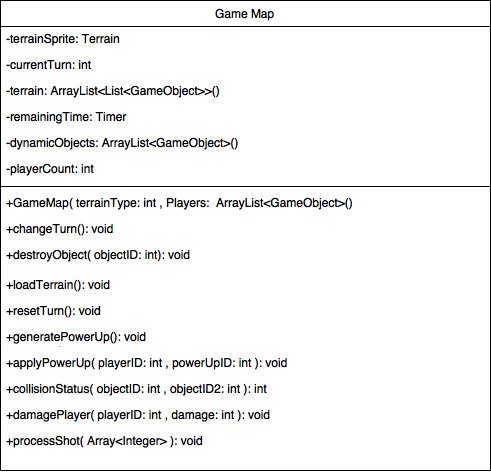
\includegraphics[width=10cm]{gamemap.png}
   \caption{GameMap Class}
   \label{fig:gamemap}
\end{figure}

\paragraph{Attributes\\}

List of attributes used in GameMap class.\\
\textbf{private terrainSprite:} This attribute stores the image file associated with the current object.\\
\textbf{private currentTurn:} This attribute stores the image file associated with the current object.\\
\textbf{private terrain:} This attribute stores the image file associated with the current object.\\
\textbf{private remainingTime:} This attribute stores the image file associated with the current object.\\
\textbf{private dynamicObjects:} This attribute stores the image file associated with the current object.\\
\textbf{private playerCount:} This attribute stores the image file associated with the current object.

\paragraph{Constructors \\}
List of constructors used in GameMap class.\\
\textbf{public GameMap:} 

\paragraph{Operations \\}
List of operations used in GameMap class.\\
\textbf{public void changeTurn:} Uses the active weapon to perform shooting operation. \\
\textbf{public void destroyObject:} Uses the active weapon to perform shooting operation. \\
\textbf{public void loadTerrain:} Uses the active weapon to perform shooting operation. \\
\textbf{public void resetTurn:} Uses the active weapon to perform shooting operation. \\
\textbf{public void generatePowerUp:} Uses the active weapon to perform shooting operation. \\
\textbf{public void collisionStatus:} Uses the active weapon to perform shooting operation. \\
\textbf{public void damagePlayer:} Uses the active weapon to perform shooting operation. 

%/GameMap



%Location
\subsubsection{Location} %image is not in the right place, because latex doesn't want to waste page

Figure \ref{fig:location} illustrates the GameMap Class.
\begin{figure}[h!]
   \centering
   \vspace{10pt}%
   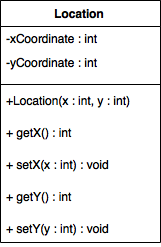
\includegraphics[width=10cm]{location.png}
   \caption{Location Class}
   \label{fig:location}
\end{figure}

\paragraph{Attributes\\}

List of attributes used in Location class.\\
\textbf{private xCoordinate:} \\
\textbf{private yCoordinate:} 


\paragraph{Constructors \\}
List of constructors used in Location class.\\
\textbf{public Location:} 

\paragraph{Operations \\}
List of operations used in Location class.\\
\textbf{public void getX:}  \\
\textbf{public void getY:}  \\
\textbf{public void setX:}  \\
\textbf{public void setY:}  


%/Location


%GameObject
\subsubsection{GameObject} %image is not in the right place, because latex doesn't want to waste page

Figure \ref{fig:gameobject} illustrates the GameObject Class.
\begin{figure}[h!]
   \centering
   \vspace{10pt}%
   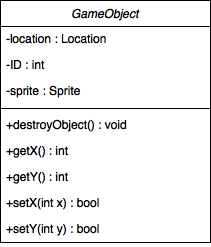
\includegraphics[width=10cm]{gameobject.png}
   \caption{GameObject Class}
   \label{fig:gameobject}
\end{figure}

\paragraph{Attributes\\}

List of attributes used in GameObject class.\\
\textbf{private location:} \\
\textbf{private ID:} \\
\textbf{private sprite:} \\

\paragraph{Operations \\}
List of operations used in GameObject class.\\
\textbf{public void destroyObject:}  \\
\textbf{public void getY:}  \\
\textbf{public void setX:}  \\
\textbf{public void setY:}  

%/GameObject


%PowerUp
\subsubsection{PowerUp} 

Figure \ref{fig:powerup} illustrates the PowerUp Class.
\begin{figure}[h!]
   \centering
   \vspace{10pt}%
   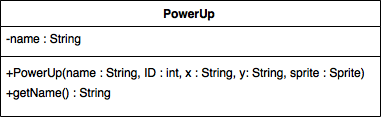
\includegraphics[width=10cm]{powerup.png}
   \caption{PowerUp Class}
   \label{fig:powerup}
\end{figure}

\paragraph{Attributes\\}

List of attributes used in PowerUp class.\\
\textbf{private name:} This attribute stores the name of the specific power up.

\paragraph{Constructors \\}
List of constructors used in PowerUp class.\\
\textbf{public PowerUp:} This constructor retrieves name, ID, coordinates, texture file from its parameter and sets necessary values accordingly.

\paragraph{Operations \\}
List of operations used in PowerUp class.\\
\textbf{public String getName:} This operations retrieves the name of the powerup and returns it as a String.


%/Location


%player
\subsubsection{Player} %image is not in the right place, because latex doesn't want to waste page

Figure \ref{fig:player} illustrates the Player Class.
\begin{figure}[h!]
   \centering
   \vspace{10pt}%
   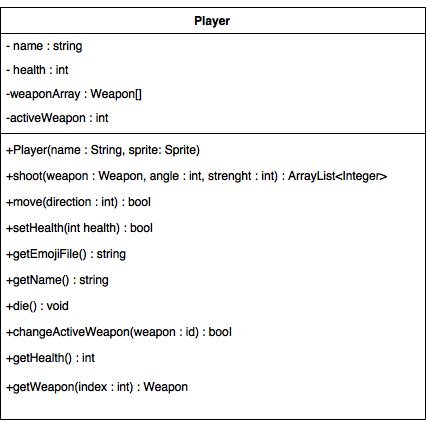
\includegraphics[width=10cm]{player.png}
   \caption{Player Class}
   \label{fig:player}
\end{figure}

\paragraph{Attributes\\}

List of attributes used in Player class.\\
\textbf{private name:} The variable which holds the prompted name of the user.\\
\textbf{private health:} The variable which holds the health value of the player.\\
\textbf{private weaponArray:} This attribute holds the weapon objects available to the specific player.\\
\textbf{private activeWeapon:} This attribute holds the weapon currently selected by the current player.

\paragraph{Constructors \\}
List of constructors used in Player class.\\
\textbf{public Player:} Initializes Player object's attributes which are name, health, weaponArray, activeWeapon. It takes name as its parameter.

\paragraph{Operations \\}
List of operations used in Player class.\\
\textbf{public void Shoot:} Uses the active weapon to perform shooting operation. Returns an arraylist of values resulting from the shooting operation to be used later.\\
\textbf{public void move:} Moves the player in one of the four degrees of freedom.  It takes direction as integer parameter. \\
\textbf{public void setHealth:} Sets health to prompted health value obtained in parameter. \\
\textbf{public String getEmojiFile:} Retrieves the file path of the emoji file sprite. \\
\textbf{public String getName:} Retrieves the name of the player. \\
\textbf{public void die:} Triggers the \textit{removeObject} method of the \textit{GameMap} class. \\
\textbf{public void changeActiveWeapon:} Changes the current active weapon to the desired weapon specified by the integer id in the parameter. \\
\textbf{public int changeActiveWeapon:} Retrieves the health value of the player. \\
\textbf{public Weapon getWeapon:} Retrieves the Weapon object currently used by the player. 

%/player


%Weapon
\subsubsection{Weapon} %image is not in the right place, because latex doesn't want to waste page

Figure \ref{fig:weapon} illustrates the Weapon Class.
\begin{figure}[h!]
   \centering
   \vspace{10pt}%
   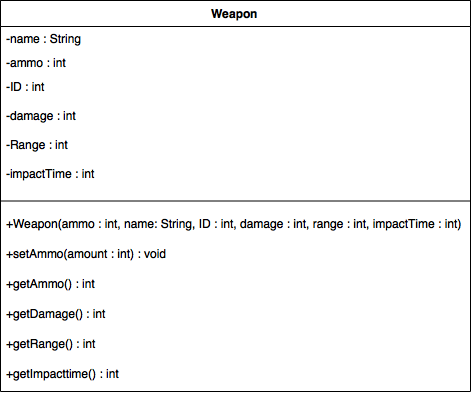
\includegraphics[width=10cm]{weapon.png}
   \caption{Weapon Class}
   \label{fig:weapon}
\end{figure}

\paragraph{Attributes\\}

List of attributes used in Weapon class.\\
\textbf{private name:} The variable which holds the prompted name of the weapon.\\
\textbf{private ammo:} The variable which holds the ammo value of the weapon.\\
\textbf{private ID:} This attribute holds the primary ID of the weapon.\\
\textbf{private damage:} This attribute holds the damage value of the weapon.\\
\textbf{private range:} This attribute holds the range of the weapon, determining the maximum distance it can travel. \\
\textbf{private impactTime:} This attribute determines the amount of time specific weapon will spend during the projectile motion. \\

\paragraph{Constructors \\}
List of constructors used in Weapon class.\\
\textbf{public Weapon:} Initializes Weapon class's attributes name, ammo, ID, damage, range, impactTime.

\paragraph{Operations \\}
List of operations used in Weapon class.\\
\textbf{public void setAmmo:} Sets the ammo of the weapon to the prompted amount. \\
\textbf{public void getAmmo:} Retrieves the current ammo value of the weapon. \\
\textbf{public void getDamage:} Retrieves the current damage value of the weapon. \\
\textbf{public void getRange:} Retrieves the current range value of the weapon. \\
\textbf{public void getImpactTime:} Retrieves the current impact time value of the weapon. 

%/weapon

%Sprite
\subsubsection{Sprite} %image is not in the right place, because latex doesn't want to waste page

Figure \ref{fig:sprite} illustrates the Sprite Class.
\begin{figure}[h!]
   \centering
   \vspace{10pt}%
   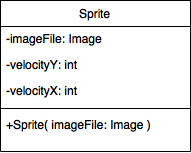
\includegraphics[width=10cm]{sprite.png}
   \caption{Sprite Class}
   \label{fig:sprite}
\end{figure}

\paragraph{Attributes\\}

List of attributes used in Sprite class.\\
\textbf{private imageFile:} This attribute stores the image file associated with the current object.\\
\textbf{private velocityX:} The variable which holds the vectorial horizontal speed value of the sprite.\\
\textbf{private velocityY:} The variable which holds the vectorial vertical speed value of the sprite.\\
\paragraph{Constructors \\}
List of constructors used in Sprite class.\\
\textbf{public Sprite:} Initializes Sprite class's attributes imageFile, velocityX, velocityY values.


%/Sprite


%management
\subsection{Management Subsystem}

Figure \ref{fig:controller} illustrates the Management Subsystem Diagram.

\begin{figure}[h!]
   \centering
   \vspace{10pt}%
   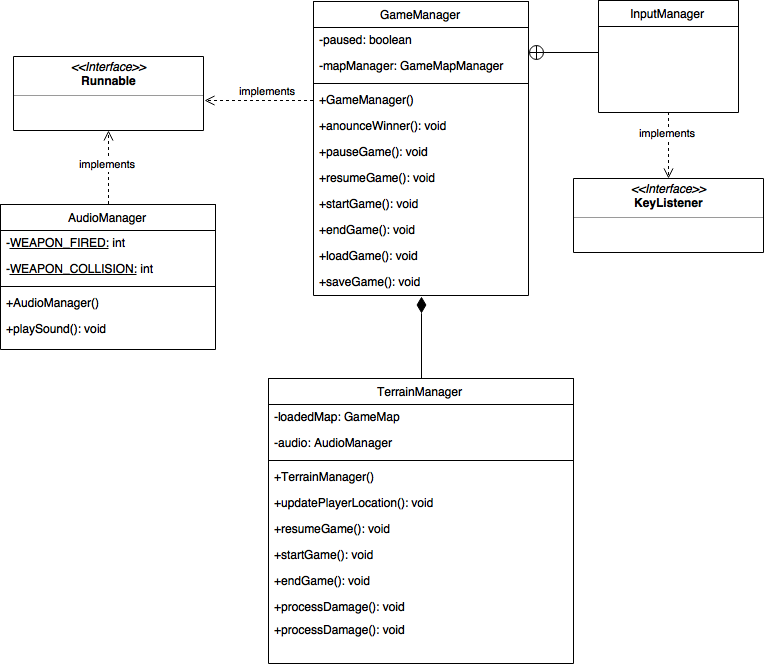
\includegraphics[width=17cm]{controller.png}
   \caption{Management Subsystem}
   \label{fig:controller}
\end{figure}


Entities Subsystem consists of 7 classes which contains the objects and information necessary to provide interactions between objects.  There is also an abstract entity used in this design.






%----------------------------------------------------------------------------------------
%	BIBLIOGRAPHY
%----------------------------------------------------------------------------------------

\pagebreak
\begin{thebibliography}{99} % Bibliography - this is intentionally simple in this template

%\bibitem[Deneme and deneme, 2009]{Figueredo:2009dg}
%Figueredo, A.~J. and Wolf, P. S.~A. (2009).
%\newblock Assortative pairing and life history strategy - a cross-cultural
%  study.
%\newblock {\em Human Nature}, 20:317--330.
 
\end{thebibliography}

%----------------------------------------------------------------------------------------

\end{document}